%
%-----------------------------------------------------------
%% Computer Music Journal LaTeX template
%%
%% September  2009
%% Author: Cornelia Kreutzer, University of Limerick


%---Document preamble
%
\documentclass[letterpaper, 12pt]{article}


% Back to the UTF-8 encoding.
\usepackage{cmjStyle} %use CMJ style
\usepackage{natbib} %natbib package, necessary for customized cmj BibTeX style
\bibpunct{(}{)}{;}{a}{}{, } %adapt style of references in text
\doublespacing
\raggedright % use this to remove spacing and hyphenation oddities
\setlength{\parskip}{2ex}
\parindent 24pt
\urlstyle{same} % make url tags have the same font
\setcounter{secnumdepth}{3} % remove section numbering
\usepackage{epstopdf}
\usepackage{amsmath,amssymb,amsbsy,bm,upgreek,nicefrac}
\usepackage{todonotes,microtype}
% For timeline/flow charts/mind maps:
\usepackage{tikz}
\usetikzlibrary{fit, calc, decorations.markings, shapes.geometric, arrows, mindmap}
\usepackage{chronosys}
%For definitions
\usepackage{enumitem}% http://ctan.org/pkg/enumitem

% Use the Figures subfolder for image files
\graphicspath{{./Figures/}}

\inputencoding{utf8}

%% ----------------------------------------------------------------------------------------------------------------------------------------
%% CMJ page headers
%% For initial submission use \lhead{Anonymous}
%% On acceptance for publication, use real author surnames for \lhead modeled on the following examples
%%		One author:	\lhead{\small Keislar}
%%		Two authors:	\lhead{\small Keislar and Castine}
%%		Three authors:	\lhead{\small Keislar, Castine, and Rundall}
%%		Four or more:	\lhead{\small Keislar et al.}
%%
\lhead{\small Grivakis}


%% The package endfloat moves all floats (figures, tables...) to the end of the article, as required for the final version of a CMJ article.
%% Leave this package commented out for initial submission, but uncomment it and the following callout commands for the final version. 
% \usepackage{endfloat}
% \renewcommand{\figureplace}{%
%	\begin{center}
%		\textbf{<<TYPE: INSERT \figurename~\thepostfig\ ABOUT HERE.>>}
%	\end{center}}
% \renewcommand{\tableplace}{%
%	\begin{center}
%		\textbf{<<TYPE: INSERT \tablename~\theposttbl\ ABOUT HERE.>>}
%	\end{center}}

%---Document----------
\begin{document}

{\cmjTitle Composition and Performance for Live Electronic Ensembles}
\vspace*{24pt}

 

% Author: name
{\cmjAuthor Athanasios Grivakis}	% List all authors here
							% e.g.:
							% {\cmjAuthor Doug Keislar, Peter Castine, and Jake Rundall}
 
% Author: address
\begin{cmjAuthorAddress}
	Georgia Tech School of Music\\
	Georgia Institute of Technology\\
	840 McMillan St NW\\
	Atlanta, GA 30332 USA\\		% Adapt as needed for non-US addresses
	agrivakis3@gatech.edu
\end{cmjAuthorAddress}

\begin{abstract}

%%% Abstract

%
This paper explores the concept of live electronic ensembles.
%
Live electronic ensembles, in the context of this paper, refers to a group of people who compose and play music together by integrating their own technology (hardware and software) with their music and performance in a manner that lacks rigidly established roles.
%
In other words, there isn't a notion of "the composer", "the hardware engineer", or "the programmer", "the performer"; each member works on all the aspects, and the members work on all the aspects together.
%
For live electronic ensembles, the use of electronic instruments and techniques serves as both a means of producing music and as an art form.
%
Starting with early influences of electronic music and experimentation with how music ought to be structured, the paper explores the innovations in musical roles and in performance technology that led to the formation of live electronic ensembles and then navigates popular examples of live electronic ensembles.
\end{abstract}

% \section{Introduction}

% %
% In this paper, the formation and practice of live electronic ensembles is explored.
% %
% Live electronic ensembles, in the context of this paper, refers to a group of people who compose and play music together by integrating their own hardware and software with their music and performance in a manner that lacks rigidly established roles.
% %

% %
% With this, some relevant questions to ask are: What is a live electronic ensemble?
% %
% What led to the formation of live electronic ensembles?
% %
% Where can examples of live electronic ensembles be seen in the culture and influence today?

% \begin{description}[font=\sffamily\bfseries, leftmargin=1cm, style=nextline]
%   \item[music]
%     Lorem ipsum dolor sit amet, consectetur adipiscing elit, sed do eiusmod tempor incididunt ut labore et dolore magna aliqua.
%   \item[experimental classical]
%     Lorem ipsum dolor sit amet, consectetur adipiscing elit, sed do eiusmod tempor incididunt ut labore et dolore magna aliqua.
%   \item[musique concrète]
%     Lorem ipsum dolor sit amet, consectetur adipiscing elit, sed do eiusmod tempor incididunt ut labore et dolore magna aliqua.
%   \item[electronic music]
%     Lorem ipsum dolor sit amet, consectetur adipiscing elit, sed do eiusmod tempor incididunt ut labore et dolore magna aliqua.
%   \item[computer music]
%     Lorem ipsum dolor sit amet, consectetur adipiscing elit, sed do eiusmod tempor incididunt ut labore et dolore magna aliqua.
%   \item[live electronic music]
%     Lorem ipsum dolor sit amet, consectetur adipiscing elit, sed do eiusmod tempor incididunt ut labore et dolore magna aliqua.
%   \item[live electronic ensemble]
%     Lorem ipsum dolor sit amet, consectetur adipiscing elit, sed do eiusmod tempor incididunt ut labore et dolore magna aliqua.
%   \item[electroacoustic music]
%     Lorem ipsum dolor sit amet, consectetur adipiscing elit, sed do eiusmod tempor incididunt ut labore et dolore magna aliqua.
%   \item[laptop orchestra]
%     Lorem ipsum dolor sit amet, consectetur adipiscing elit, sed do eiusmod tempor incididunt ut labore et dolore magna aliqua.
%   \item[network music]
%     Lorem ipsum dolor sit amet, consectetur adipiscing elit, sed do eiusmod tempor incididunt ut labore et dolore magna aliqua.
% \end{description}

\vspace*{24pt}
 
\section{Music Leading up to Live Electronic Ensembles}

This section explores the origins of live electronic ensembles and the musical movements, and people that influenced how live electronic ensembles came to be. To this end, it is necessary to investigate the history of the music that paved the way for live electronic ensembles and live electronic music.

%
From the late 1800s to the 1940s, there was a wave of experimentation with music composition and with music recording.
%
The idea of how music ought to be defined was set to encompass the notion of organized noise and sounds, as opposed to earlier notions from traditional and classical music.
%
Musicians started experimenting with using sounds to create music and recording sounds on tape recorders and magnetic tapes.
%
Some important people involved were Edgard Varèse, Walter Ruttman, and Halim El-Dabh.

%
During the 1940s and 1950s, Pierre Schaeffer and Pierre Henry pioneered musique concrète, later influencing the Studio for Electronic Music of the West German Radio in Cologne.
%
This influence eventually extended to people such as Olivier Messiaen and Karlheinz Stockhausen, the latter of whom experimented with serialism music structure and who pioneered electronic music.
%

%
Also during the 1940s and 1950s, electronic music was experimented with in the United States.
%
Groups of a few experimental composers and performers began to tinker with circuits, early forms of networks, loudspeakers, transistors, and other related technologies.
%
These people experimented with making their own musical devices and performing musical compositions together before synthesizers and electronic instruments were commercially available.
%
Some key people involved were John Cage, David Tudor, Gordan Mumma, and Robert Ashley.
%

%
Around the 1950s and 1960s, computer music and electronic music technology began to become significant.
%
Around 1950, CSIRAC was the first electronic computer to play digital music.
%
A student of Messiaen, Iannis Xenakis experimented with a music structure known as stochastic music and developed mathematical and computation models to aid in music composition.
%
John Cage’s 1951 piece Imaginary Landscape No. 4 for Twelve
Radios was one of the earliest examples of an experimental
networked music performance, making use of interconnected radio transistors.
%
Stockhausen during this time became famous for experimenting with using microphones as instruments and for using electronic generators and modulators as early examples of live electronic music.

%
At MIT Bell Labs during the 1960s and 1970s, Max Mathews and Jean-Claude Raoul Olivier Risset worked on computer sound synthesis and developed music software for producing standard digital audio.
%
They were also involved with ICRAM and served there as administrators.
%
In the 1970s, a student of Messiaen named Pierre Boulez founded ICRAM, which became a research center where people such as John Chowning and Max Mathews worked.
%
ICRAM was later influential to groups such as the computer network band The Hub.
%
John Chowning experimented with FM synthesis, which along with affordable digital chips, enabled realistic electronic music and allowed for real-time performance to become more affordable and widespread.
%
In the 1970s, Chowning founded CCRMA, which became a hub for musicians, composers, researchers, and engineers to collaborate and use computer-based technology as an artistic medium and as a research
tool.

%
From the 1970s onward, live electronic bands have been performing music using electronics and technology in real time.
%
The German band Kraftwerk is one major example of such a band.
%
Kraftwerk is known for pushing the technological and performance boundaries in live music performance and discussed their vision of portable computers being part of live music performance and culture in a 1991 interview.

\vspace*{24pt}

\subsection{Early 1900s}

\subsubsection{Early Compositions and Recording Experimentation} % earli(est) examples

During the first half of the 20\textsuperscript{th} century, a wave of musical composers and musicians began experimenting with taking music in different directions from traditional classic music.

%%% Edgard Varèse

%
During the earliest parts of the 20th century, the French composer Edgard Varèse explored notions of "organized sound", and emphasized concepts such as timbre and rhythm in his music. 
%
Varèse came up with a definition of music in accordance to his views of music as "organized sound": Varèse viewed "sound as living matter" and "musical space as open rather than bounded" \citep{wen1966open}.
%
Varèse organized his music according to "sound-masses", viewing this structure as mimicking the structure of crystals in nature \citep{wen1966varese}.
%
Varèse thought that "to stubbornly conditioned ears, anything new in music has always been called noise", and he posed the question, "What is music but organized noises? \citep{varese1966liberation}"
%
From his early explorations of music, Varèse can be said to have influenced later composers such as John Cage, Olivier Messiaen, Pierre Boulez, Karlheinz Stockhausen, and Iannis Xenakis, among others.

%%% Arnold Schoenberg and serialism

%
Throughout the early 20th century, serialism became popular among experimental musicians.
%
Originating with Arnold Schoenberg's twelve-tone technique, serialism was a methodical way of composing music involving post-tonal musical composition and manipulating pitches, rhythms, dynamics, and timbres with intentional structure.
%
Serialism was influential to many early predecessors of electronic music, such as John Cage, Olivier Messiaen, and Karlheinz Stockhausen, among others.

%%% Walter Ruttman

%
Walter Ruttman was a German cinematographer and film director who was instrumental in abstract filmmaking and experimental music during the 1920s. 
%
Ruttman served in WW1, from which he suffered from PSTD. Ruttman later started making avant-garde films.
%
It is suggested that Ruttman sympathized with Nazism; along the lines of Nazi ideology, Ruttmann showed in some of his films that harmony and tradition prevailed over the modern city that had taken over \citep{goergen1989walter}.
%
In the early 1920s, Ruttman experimented with films such as \textit{Opus I} and \textit{Opus II}, which displayed abstract geometric shapes and colorful kaleidoscopic patterns.
%
Ruttman directed the semi-documentary 'city symphony' silent film \textit{Berlin: Symphony of a Metropolis} in 1927. 
%
As Ruttman himself put it, "Since I began in the cinema, I had the idea of making something out of life, of creating a symphonic film out of the millions of energies that comprise the life of a big city." \citep[p. xxx]{dormehl2012journey}
%
Presented in 1930, Ruttman's work \textit{Wochenende (Weekend)} was an audio montage considered influential in the development of audio plays and considered a pioneering work of musique concrète.
%
Filmed using the Tri-Ergon process, the montage features audio of street sounds of Berlin captured with a camera without images, as this was before magnetic tape  \citep{williams2017concrete}, \citep{segel2002transparent}.

\subsection{1940s to 1950s}

\subsubsection{Electroacoustic Tape Music}

%%% Halim El-Dabh

%
Halim El-Dabh was an Egyptian-American composer, musician, and ethnomusicologist active during the 1940s.
%
El-Dabh realized sound recordings could be used as raw materials to create music. 
%
El-Dabh experimented with electronic music as a student in Cairo in the early 1940s, where he manipulated sounds with wire recorders.
%
El-Dabh played around with reverberation, echo chambers, voltage controls, and a re-recording room with movable walls to create varying levels of reverb.
%
It was in the streets of Cairo that El-Dabh recorded sounds from an ancient zaar exorcism ritual, hoping to manipulate the recorded sounds to open up the "inner sound" contained within \citep{holmes2008electronic}.
%
El-Dabh's 1944 work \textit{The Expression of Zaar} was one of earliest known magnetic tape music and works of musique concrète, pre-dating Pierre Schaeffer's work by four years \citep{holmes2008electronic}.
%
El-Dabh was a supporter of civil rights and experienced racism from having a darker skin tone, and his ties to African American culture were deepened when he taught music at Howard University. \citep{seachrist2003musical}.

\subsubsection{Musique Concrète}

%%% Pierre Schaeffer

%
Pierre Schaeffer was a French composer, writer, broadcaster, engineer, musicologist, and acoustician during the 1950s, and founder of Groupe de Recherche de Musique Concrète (GRMC).
%
Schaeffer was one of the pioneers of musique concrète ("concrete music"), a term he coined in 1948 \citep{schaeffer1992pierre}.
%
Schaeffer believed that traditional classical music began as an abstraction of musical notation that later became audible music.
%
Musique concrète, by contrast, starts with concrete sounds and then abstracts them into a composition.
%
In this sense, musique concrète is a breaking down of traditional music theory, starting from the bottom up. 
%
Schaeffer emphasized including any sounds in works of music and made early use of techniques such as tape looping and tape splicing.
%
Schaeffer was known for freely improvising sound, and this notion of electroacoustic improvisation was important later on for live electronic music.
%
Schaeffer authored \textit{Treatise on Musical Objects: An Essay across Disciplines}, in addition to several musical treatises and an array of musical works.


\subsubsection{Elektronische Musik, Germany}

%%% Elektronische Musik Studio

%
The Studio for Electronic Music of the West German Radio in Cologne was a center of electronic music innovation originally composed of physicist Werner Meyer-Eppler, sound engineer Robert Beyer, technician Fritz Onkel, and composer Herbert Eimert.
%
The studio's earliest history is a meeting held by these founding members during a tape-recorded late-night program about electronic music broadcast in 1951 \citep{morawska1988schwingende}.
%
The founding members at the time were experimenting with atonal music theory and timbre-oriented music.
%
Eimert originally served as the studio director and was later succeeded by Stockhausen in 1963.
%
Meyer-Eppler wrote about electronic music in 1949 in his book Elektrische Klangerzeugung Elektronische Musik und Synthetische Sprache.
%
The group experimented with composing music directly on magnetic tape and manipulating electronic instruments with filters, frequency bands, modulators, and oscilloscopes.
%
The studio demonstrated its first piece publicly at the New Music Festival on 26 May 1953 for the official opening of the studio \citep{morawska1988schwingende}.
%
After this, the studio began inviting young composers to experiment with electronic music in the studio.
%

%%% Karlheinz Stockhausen

%
From the 1940s, European composers sought to organize and control all aspects of music systematically.
%
In the late 1940s, the French composer Olivier Messiaen worked on organizing pitches, durations, dynamics, and timbres.
%
One of Messiaen's students, Karlheinz Stockhausen, became a pioneer of electronic music.
%

%
Stockhausen arrived at the Cologne studio in 1953 after being invited by Eimert.
%
Previously, Stockhausen had acquired experience with sound and tape editing processes while working at Schaeffer's Groupe de Recherches de Musique concrète.
%
Stockhausen had learned that pitch, duration, and amplitude could be determined accurately, but wanted to explore how timbre could fit into serial organization.
%
Stockhausen's 1957 article \textit{"... How Time Passes ..."} explored several musical ideas, including a scale of twelve tempos analogous to the chromatic pitch scale, techniques to subdivide musical intervals similar to the overtone series, statistical composition, manipulating time and duration, and other more theoretical techniques such as "action duration", "variable form", "directionless temporal field", and "polyvalent form" \citep{stockhausen2014texte}.
%
Stockhausen composed many more important articles in electronic music, such as Elektronische und Instrumentale Musik in 1958.
%
As part of his temporal theories on music, Stockhausen expanded on ideas from acoustic music and mathematical analysis to view timbre as part of the overall structure of composition.
%
He saw timbre as directly tied to overtones and viewed color, harmony and melody, meter and rhythm, dynamics, and form as tied to the general overtone structure \citep{morgan1975stockhausen}.
%
Stockhausen's compositions \textit{Mikrophonie I} and \textit{Mixtur} from 1964 actively made use of a microphone as an instrument.
%
These live-electronic works used sine-wave generators and ring modulators, with electronic transformations being accomplished during the performance as opposed to studio-produced electronic music on tape.
%
Thus, these works were early examples of live electronic music.
%

\subsubsection{Electronic Music in the United States}

%%% John Cage

%
John Cage was an American Composer, music theorist, and pioneer of electroacoustic music during the mid-1900s.
%
Cage's earliest works were short pieces for piano involving mathematical procedures without much regard for emotional appeal \citep{pritchett1996music}.
%
Cage experimented with indeterminacy music structure, which he defined as "the ability of a piece to be performed in substantially different ways" \citep{pritchett1996music}.
%
With regards to indeterminacy, Cage claimed that "any part of a musical work is indeterminate if it is chosen by chance, or if its performance is not precisely specified. The former case is called 'indeterminacy of composition'; the latter is called 'indeterminacy of performance'" \citep{simms1996music}.
%
Cage employed a method of using hexagrams from the Chinese classical text \textit{I Ching} in addition to star charts to systematically determine by chance chance all of the components for a given musical composition, including accidentals, clefs, modes, transpositions, and playing techniques in a number of his music pieces \citep{kostelanetz2003conversing}, \citep{nicholls2002cambridge}.
%
Cage identified as an anarchist; he purposefully wrote very difficult etudes to convey the point that the impossible is not impossible (in reference to his political and social views) \citep{perloff1994john}.

%
Cage's \textit{Imaginary Landscape No. 1} (1939) was the first electroacoustic music piece produced, while also being one of earliest examples of musique concrète \citep{silverman2012begin}.
%
For this musical work, Cage made extensive use of variable and constant frequency tones and sound manipulation.
%
\textit{Imaginary Landscape No. 1} was widely used, including in a ballet called \textit{Horror Dream} for its ghastly, infernal sound qualities.
%
Cage's 1951 piece \textit{Imaginary Landscape No. 4 for Twelve Radios} by composer John Cage was one of the earliest examples of an experimental networked music performance.
%
The piece used interconnected radio transistors which were influencing each other as a musical instrument.
%
Since the radio transistors were affecting one another, this can be thought of as a network over which real-time instruments affected each other at different spatial locations.

%%% David Tudor

%
David Tudor was an American pianist and experimental composer during the early 1900s.
%
Tudor worked closely with Cage on many of Cage's pieces throughout the 50s and 60s, both works for piano and electronic pieces \citep{newworldrecords2006david}.
%
Tudor created electronic works and made musical circuits that were instrumental examples of early electronic instruments and electronic music.
%
Tudor and Gordon Mumma collaborated on a series of musical projects titled \textit{Rainforest}.
%
Tudor's 1973 \textit{Rainforest IV} was an electroacoustic sound installation that used a metal barrel, a vintage computer disk, and plastic tubing which served as a musical accompaniment.
%
In the performance, each composer designs and constructs sculpted figures that double over as instrumental loudspeakers when manipulated \citep{newworldrecords2006david}.
%
\textit{Rainforest IV} has been installed in thirty sites throughout the United States and Europe, including museums, universities, and television studios.

%%% Gordon Mumma

%
Gordan Mumma is an American composer known for self-made electronic builds and for collaborating with Tudor, Cage, and American composer Robert Ashley.
%
Mumma and Ashley co-founded the ONCE group with George Cacioppo, Roger Reynolds, and Donald Scavarda \citep{newworldrecords2006david}.
%
The ONCE Group was a space for musicians, visual artists, architects, and filmmakers to collaborate and share ideas for projects in the late 1950s and early 1960s.
%
Ashley directed the ONCE Group from 1964 to 1969 \citep{ashley2017biography}.
%
ONCE group would host the ONCE Festival of New Music in Ann Arbor, Michigan between 1961 and 1966 \citep{newworldrecords2006david}.
%
The festival facilitated development in acoustic and electronic music as well as dance, film, and multi-media performances.

%%% Robert Ashley

%
Robert Ashley was a distinguished figure in American contemporary music.
%
Ashley is well-known for his work in new forms of opera and multi-disciplinary projects.
%
The Space Theater, a loft specially designed and outfitted for performances with projected images and music from 1957 to 1964, asked  Mumma and Ashley to create live electronic music for their productions.
%
Mumma and Ashley's performances included music produced by rubbing stones together and throwing steel rings along wires \citep{holmes2002electronic}.
%
While working together for Space Theater in 1958, Ashley and Mumma created the Cooperative Studio for Electronic Music.
%
They used spare rooms in their houses for their studio, which also contained their equipment.
%
Ashley and Mumma tinkered with electronics, working before synthesizers and electronic musical instruments were commercially available.
%
They invented and built much of their own equipment with materials from electronics stores.
%
Ashley and Mumma were two of the earliest composers to work in live generation of music with amplified small sounds \citep{holmes2002electronic}.

\subsection{1950s to 1960s}

\subsubsection{Computer Music}

%%% CSIRAC

%
CSIRAC \citep{doornbusch2004computer} was Australia's first digital computer, built around 1949.
%
CSIRAC could play music from stored instructions programmed by Geoff Hill, making it the first computer to play digital music.
%
In 1950 CSIRAC was demonstrated playing music, making CSIRAC the first exhibited instance of an electronic computer playing digital music.
%
The music was never recorded, but it has been accurately reconstructed.

\subsubsection{Stochastic Music}

%%% Iannis Xenakis

%
Iannis Xenakis was a Romanian-born Greek-French avant-garde composer, music theorist, architect, performance director, and engineer during the 50s and 60s.
%
Xenakis came from an affluent background; his mother knew music, and he was educated in math, science, classics, and music.
%
Xenakis lost his mother when he was 5 years old.
%
Xenakis joined resistance movements during his college years and got hit by shrapnel from a tank.
%
Xenakis later left Greece for Paris, for which he expressed guilt; that guilt fueled his motivation to pursue music \citep{varga1996conversations}.
%
Xenakis studied classical music and sought to experiment with his music like Debussy and Stravinsky. 
%
He got rejected by numerous teachers, and later gained a deep understanding of Western music.
%
He was inspired by Greek folk and church music.
%
Xenakis, like Pierre Boulez and Stockhausen, was taught by Messiaen. 
%
Xenakis contributed to Metastaseis and later criticized Stockhausen and Boulez over their adamancy with serial music, which he felt was steering music to a dead-end \citep{slabihoudek2022sound}.
%
Xenakis eventually joined Groupe de Recherches de Musique Concrète, a music concrète group established by Schaeffer and Pierre Henry.
%
During the 60s, Xenakis began researching computer-assisted composition.
%
He applied mathematical concepts and modeling in his music, forming what is known as stochastic music.
%
In 1977, he developed UPIC, a computer system that could translate graphical images into musical results \citep{hugill2018digital}.
%
Xenakis demonstrated his music as being composed according to systematic methods while still displaying a powerful emotional feel \citep{service2013guide}.

\subsection{1960s to 1980s}

\subsubsection{MIT Bell Labs}

%%% Max Matthews

%
Max Mathews was an American pioneer of computer music who created many computer music contributions during the 60s.
%
Mathews studied electrical engineering at Caltech and MIT.
%
At Bell Labs, Mathews developed MUSIC, the first computer program that implemented direct synthesis to create digital audio waveforms \citep{clarke2020inside}.
%
MUSIC produced standard digital audio using a method of digitally representing sampled analog signals called pulse-code modulation (PCM).
%
Among Mathew's technological innovations for music are a graphic system to convert drawings to sound and GROOVE, a fully developed music synthesis system using 3C/Honeywell DDP-24 minicomputers, a CRT display, 12bit D/A for real-time sound playback, an interface for analog devices, a musical keyboard, knobs, and rotating joysticks \citep{bogdanov2001all}.

%%% Jean-Claude Raoul Olivier Risset

%
Jean-Claude Raoul Olivier Risset was a French composer who made pioneering contributions to computer music during the 60s and 70s.
%
Between 1964 and 1969, Risset spent time in the United States and had the opportunity to meet Edgard Varèse \citep{warszawski2013risset}.
%
Risset collaborated with Mathews at the Bell Telephone Lab on computer sound synthesis projects such as the imitation of instrumental sounds, paradoxical sounds, and sound development processes \citep{warszawski2013risset}.
%
Risset used Mathews' MUSIC IV software to recreate brass instrumental sounds in 1964 digitally.
%
Risset made digital recordings of trumpets and studied their timbral composition using spectrum analysis tools.
%
Risset also performed the earliest experiments with FM synthesis and waveshaping \citep{ircam2021risset}.
%
Risset was the head of the Computer Department at IRCAM from 1975 to 1979, and was one of its original administrators along with Vinko Globokar, John Chowning, and Max Mathews.

\subsubsection{IRCAM}

%%% Pierre Boulez

%
One of Messiaen's students, Pierre Boulez, founded the Institute for Research and Coordination in Acoustics/Music (IRCAM) in the 1970s.
%
IRCAM became a French music research institute known for avant-garde and electro-acoustical music.
%
It also became a hub for many key people such as John Chowning, who worked on FM synthesis, and Max Matthews.
%
They, along with Vinko Globokar and Jean-Claude Risset, were the original administrators of the Institute for Research and Coordination in Acoustics/Music (IRCAM).
%
IRCAM became a prominent hub for avant-garde and electro-acoustical art music, influencing later musicians, composers, and music technology.

\subsubsection{CCRMA}

%%% John Chowning

%
John Chowning is an American musician, discoverer, and professor.
%
Chowning founded the Center for Computer Research in Music and Acoustics (CCRMA) at Stanford University in 1975.
%
At CCRMA, musicians, composers, researchers, and engineers collaborate and use computer-based technology as an artistic medium and as a research tool.
%
Various musicians and engineers have worked at CCRMA, including Max Mathews (who was made a professor emeritus).
%
Chowning developed the frequency modulation, or FM, synthesis algorithm in 1967 at CCRMA \citep{chowning1973synthesis}.
%
FM synthesis allows for the production of audio signals by modulating the frequency of the waveform with a modulator.
%
Chowning figured out how to simulate a host of instrumental sounds, including singing using FM synthesis.
%
FM synthesis, which Stanford later licensed to Yamaha, brought over 20 million dollars to the university \citep{grove1980new}.
%
This made the FM synthesis patent the second-most profitable licensing agreement in Stanford's history before 1994 \citep{stanford2011music}.
%
Chowning's FM algorithms and the arrival of fast, inexpensive digital chips allowed for realistic percussion and bell-like sounds and made real-time live composition possible and affordable.
%
Chowning's 1972 work \textit{Turenas} demonstrated the ability to simulate sound motion through physical space \citep{chowning1972method}.
%
\textit{Turenas} gave the illusion of continuous 360-degree space using four strategically placed speakers \citep{grove1980new}.
%
Chowning's FM synthesis made its way to musical instruments; in 1983, Yamaha made their first commercially successful digital FM synthesizer, the DX7.

\subsection{1970s to 1990s}

\subsubsection{Kraftwerk}

%%% Kraftwerk

%
Kraftwerk is a German electronic band formed in Düsseldorf in 1970.
%
Founded by Ralf Hütter and Florian Schneider, Kraftwerk is known for its innovation and expansion of electronic music.
%
Kraftwerk is an early example of a band that popularized the genre of electronic music and is an example of krautrock music.
%
Krautrock is a music style that blends elements of psychedelic rock, avant-garde composition, and electronic music and features hypnotic rhythms, extended improvisation, musique concrète techniques, and early synthesizers.
%
Kraftwerk emerged from West Germany's krautrock scene during the early 1970s and later used electronic instrumentation such as synthesizers, drum machines, and vocoders.
%
Kraftwerk was influenced heavily by film music, classical music, German electronic music, and in machine-generated rhythm patterns.

%
On commercially successful albums such as \textit{Autobahn} in 1974, \textit{Trans-Europe Express} in 1977, \textit{The Man-Machine} in 1978, and \textit{Computer World} in 1981, Kraftwerk developed a self-described "robot pop" style that combined electronic music with pop melodies, sparse arrangements, and repetitive rhythms.
%
Kraftwerk's songs express the paradox in modern city living of feeling alienated yet simultaneously being connected to ultramodern technology \citep{barr2013kraftwerk}.
%
In an interview with British music journalist and broadcaster Jon Savage in May 1991, members of Kraftwerk stated that during their early formation: "You had these performances from Cologne radio, Stockhausen, and something new was in the air, with electronic sounds, tape machines. We were a younger generation, we came up with different textures" \citep{savage2012interview}.
%
In the same interview, Kraftwerk in response to the question "What do you think the future of music is going to be?" stated:
\begin{quote}
I do think we’re in a new musical age. We’re in the middle of a revolution, there’s one phase already finished. Miniaturisation is continuing. Trans Europe Express was done with huge machinery, and all this smaller stuff, transportable computers, will be great. We’re still carrying a lot of weight from city to city. We’re dreaming of carrying a briefcase from place to place with a laptop, little samples - little keyboards can be done already \citep{savage2012interview}.
\end{quote}
%
Despite Kraftwerk's use of digital and computer-controlled sequencing in its performances, live performance has always played an important role.
%
Kraftwerk has developed a reputation of reclusivity, with occasional interviews and answers to fans.

%
Throughout their career, Kraftwerk has pushed the limits of music technology with some notable innovations, such as homemade instruments and custom-built devices.
%
One example of this is Kraftwerk used a custom-built vocoder on their albums \textit{Ralf und Florian} and \textit{Autobahn} \citep{moogulator2006vocoder}.
%
Alexei Monroe called Kraftwerk the "first successful artists to incorporate representations of industrial sounds into non-academic electronic music" \citep{monroe2005interrogation}.
%
AllMusic wrote that their music "resonates in virtually every new development to impact the contemporary pop scene of the late 20th century" \citep{allmusic2009kraftwerk}.

%
The group has had nearly 30 different lineups from 1970 to present day. Some of the roles of members have included the following: vocals, flute, guitar, keyboards, bass, violin, drums, electronic percussion, video technician, and studio album.
%
Currently, the members are:
Ralf Hütter on lead vocals, vocoder, synthesizers, and keyboards,
Henning Schmitz on sound effects, and live keyboards,
Falk Grieffenhagen on electronic percussion, and
Georg Bongartz on live video technician \citep{monteiro2023c6}.

\section{Emergence of Live Electronic Ensembles}

The experimentation with musical structure and innovation of technology in music was instrumental in the emergence and development of live electronic ensembles.
%
This next section will explore what a live electronic ensemble is and the philosophy of live electronic ensembles. This section will also delve into examples of live electronic ensembles such as computer network music bands and laptop orchestras.
%
Network music refers to a real-time interaction over a computer network that lets musicians in different locations perform together as if they were physically next to each other.
%
Network music expanded with the band The Hub and with the SoundWIRE research group at CCRMA, and is influential in the area of laptop orchestras.
%
Laptop orchestras feature a group of musicians, composers, and engineers playing together primarily using laptops as the instruments and medium for playing and creating music.

\vspace*{24pt}

\subsection{Computer Network Music}

\subsubsection{The Hub}

%%% The Hub

%
As personal computers became more available and affordable in the late 1970s, groups of people involved in experimental and electronic music began linking multiple computers, electronic instruments, and analog circuitry to create novel forms of music.
%
One notable example is the League of Automatic Music Composers, formed by John Bischoff, Tim Perkis, Jim Horton, and Rich Gold.
%
While collaborating at a performance at The Network Muse Festival in 1986 at The LAB in San Francisco, Perkis and Bischoff were playing around with their music and tech equipment \citep{brown2002indigenous}.
%
Rather than implement an ad-hoc wired connection of computer interaction for a performance, they decided to try using a hub, meaning a general purpose connection for network data.
%
This method was less failure-prone and enabled greater collaborations \citep{brown2002indigenous}.

%
Considered the first computer network band, The Hub is an American computer network music ensemble formed in 1986 which grew from the League of Automatic Music Composers.
%
Its members are John Bischoff, Tim Perkis, Chris Brown, Scot Gresham-Lancaster, Mark Trayle and Phil Stone \citep{bischoff2002indigenous}, \citep{brown2002indigenous}.
%
The Hub is the first live computer music band whose members are all composers who design and build their hardware and software \citep{gresham1999aesthetics}.
%
The Hub experimented in 1997 with sending MIDI data over Ethernet to distributed locations.
%
Reportedly, “it was more difficult than imagined to debug all of the software problems on each of the different machines with different operating systems and CPU speeds in different cities”.
%
The Hub is also the first band to do a telematic performance in 1987 at the Clocktower in New York \citep{brown2002indigenous}.
%
Because this work is among the earliest in the live music practice of networked music performance, they are a characteristic example of a network ensemble in computer music \citep{collins2010introduction}.
%
The Hub's best-known piece, \textit{Stuck Note} by Scot Gresham-Lancaster has been covered by a number of network music bands, including several laptop orchestras: the Milwaukee Laptop Orchestra (MiLO), and the Birmingham Laptop Ensemble (BiLE) \citep{surges2008networking} \citep{bilemusic2012all}.

%
Jon Bischoff discusses his approach to composition and software in his article \textit{Software as Sculpture: Creating Music from the Ground Up}.
%
\begin{quote}
In programming a computer to generate music, distinctive characteristics and limitations of the computer medium
are inevitably revealed in the sonic behavior of the program.
These characteristics might include timing complexities,
effects created by sudden transitions in loudness or pitch,
or unforeseen artifacts that are the result of the unique flow
of the program. As these features arise and become part of
the musical process, the composer/programmer is brought
into contact with the fundamental nature of the computer
as a musical instrument" \citep{bischoff1991software}.
\end{quote}
%
He also discusses how he applied this to two compositions, \textit{Audio Wave} and \textit{Next Tone, Please}.
\begin{quote}
The process by which the pieces [\textit{Audio Wave} and \textit{Next Tone, Please}] were constructed is characterized by
bottom-up design and the empirical method. Starting from
an initial idea or perception, I composed each piece by
adding a feature at a time, making aesthetic choices by
repeated close listening. As a result of this process, some
features were refined, others were dropped. Finally, the
identity of each piece emerged. Although this way of working within a medium is common in visual art, it is unusual
within the field of computer programming. It is generally
thought that programmers implement their ideas on the
computer with as few unforeseen developments as possible,
and that ideas flow in only one direction, from the operator
to the machine. From the vantage point of an artist, though,
it is just as easy to see the flow going in the opposite direction: the medium reveals itself as the artist proceeds, and
such revelations shape the direction in which the artist
continues. This interaction between artist and medium, and
the intimacy it suggests, is no different for a computer artist \citep{bischoff1991software}.
\end{quote}
%
In this article, Bischoff mentions that \textit{Next Tone, Please} grew out of his involvement with the music of Charles
Ives, which was introduced to him by James Tenney.
%
Bischoff studied with Tenney at the California Institute of the Arts, 
from 1970 to 1971 \citep{bischoff1991software}.

%
Another one of the members of The Hub, Tim  Perkins, made the following statement on his guiding philosophy on his personal website:
\begin{quote}
I like to consider human-machine interaction as a new form of social interaction. What's interesting to me about computers is their ability to serve as a framework for embodying systems offering complexity and surprise. Unpredictability is what makes social life so interesting, it is what makes art so interesting, and it's what can make computers, as partners in art making, interesting. I don't use computers to simply carry out ideas I may have: I'd rather work in situations that force me to respond to surprises that are dealt to me by systems whose complexity and unpredictability are so high that their behavior can not be known in advance. All of my computer based art work has been concerned with creating social (or synthetic social) situations, which have enough complexity to behave like real life: in fact, to be real life of some new kind. The system in question in almost all of these pieces consists of human beings and machines in cycles of mutual influence and response \citep{perkins2024about}.
\end{quote}

\subsubsection{SoundWIRE at CCRMA}

%%% SoundWIRE

%
The development of high-speed internet through groups such as Internet2 led to high-quality audio links beginning in the early 2000s.
%
One of the first research groups to take advantage of the improved network performance was the SoundWIRE research group at Stanford University's CCRMA \citep{chafe2000simplified}.
%
SoundWIRE is concerned with the use of Internet networks as an extension to computer music performance, composition, and research.
%
SoundWIRE research uses Internet2 and other countries' high-speed/bandwidth networks.
%
According to SoundWIRE's website, research areas include professional-quality multi-channel Audio streaming, Internet physical models and virtual acoustics, sonification of network reliability, human factor (psychoacoustics) in network performance, and Internet/computer/acoustic music performance practice \citep{caceres2007soundwire}.
%
With an exponential increase in computer and network speed, low-latency multichannel streaming is already possible with speeds approaching the physical speed limit of light waves \citep{caceres2007soundwire}.
%
SoundWIRE believes that next-generation computer music will experience new possibilities that enhance network performance, composition, and acoustical space \citep{caceres2007soundwire}.
%
SoundWIRE has collaborated in music and research with several global institutes, including Banff Centre in Alberta, Canada, Rensselaer Polytechnic Institute (RPI) in Troy, New York, Sonic Arts Research Centre (SARC) in Belfast, Northern Ireland, and the University of Santa Cruz (UCSC) at Santa Cruz, California \citep{caceres2007soundwire}.


\subsection{Laptop Music}

\subsubsection{Laptronica}

%%% Laptronica

%
In the early 1990s, Laptronica became a popular form of live electronic music in which laptops were used as instruments.
%
Laptronica was significant because highly efficient and portable computation became available to musicians, leading to its usage in live performances.
%
Methods of sound production, manipulation, and organization previously inaccessible outside of music studios and academia became available for use in live performances. They were, in particular, popular with younger musicians who were both influenced by and interested in experimental music forms \citep{emmerson2017living}.
%

\subsubsection{Farmers Manual}

%%% Farmers Manual

Also during the beginning of the 1990s, an electronic music and visual art group called Farmers Manual was founded in Vienna.
%
The group includes Mathias Gmachl, Stefan Possert, Oswald Berthold, Gert Brantner, and Nik Gaffney.
%
Farmers Manual was part of the Viennese electronic music scene of the 1990s.
%
The group members consist of musicians, DJs, computer geeks, and net freaks who count music as only one of several ongoing projects \citep{cooper2024farmers} \citep{allmusic2024farmers}.
%
The group bounces between electronic music, live visuals, experimental graphics, and web design.
%
According to their entry on the online record store and music community website Bandcamp: "farmersmanual is a self-generating memeplex lazily self-organised around the enterprise of doped-out electronics... since 1996 it has been evolving as a subsurface autopoetic process with erratic overt activity consistently transmitting a unique quality of pathology and beauty skimming the bow-wave of mainstream aesthetics" \citep{bandcamp2024farmers}.
%
The group's identity is shrouded in mystery, even though their releases have garnered an international audience \citep{cooper2024farmers} \citep{allmusic2024farmers}.
%
Farmers Manual emphasizes live performances and has released albums through avant-garde labels Mego, Tray, and Or \citep{last2014farmers}.
%
The group's full-length debut, \textit{No Backup}, is a collection of "drawn-out discombobulations of standard rhythmic and melodic structures" \citep{cooper2024farmers} \citep{allmusic2024farmers}.
%
The group has also experimented with drum'n'bass-style rhythmic programming and has conducted live Internet broadcasts via their website: \textit{farmersmanual.co.at} \citep{cooper2024farmers} \citep{allmusic2024farmers}.

\subsubsection{Laptop Orchestra}

%%% Laptop Orchestra

%
The combination of many laptops in live performance led to the formation of laptop orchestras.
%
A laptop orchestra is a chamber music ensemble consisting of musicians, engineers, and composers making music primarily through laptops.
%
Laptop orchestras first appeared in the United States at universities.
%
PLOrk (Princeton Laptop Orchestra) was founded by Dan Trueman and Perry Cook in 2005 \citep{snyder2022about}.
%
PLOrk started the laptop orchestra trend, first performing in 2006.
%
In PLOrk, each laptopist uses hemispherical speaker to emulates how traditional orchestral instruments cast sound in space \citep{snyder2022about}.
%
Wireless networking and video augment the familiar role of the conductor, suggesting unprecedented ways of organizing large ensembles \citep{snyder2022about}.
%
PLOrk has performed at places like Carnegie Hall and the American Academy of Sciences in DC.
%
The group is currently directed by composer and instrument designer Jeff Snyder, the Director of Electronic Music at Princeton \citep{snyder2022about}.
%
PLOrk has made extensive use of ChucK, a music programming language created by Ge Wang and Perry Cook that enables performers to develop new code in preparation and performance.
%
According to Trueman, PLOrk differed from preceding ensembles such as The Hub, where the players each design their instruments individually.
%
In contrast with The Hub, "PLOrk is a collection of meta-instruments whose players might change from piece to piece" \citep{trueman2007laptop}.
%
Trueman also discussed that PLOrk is more than a live electronic ensemble; in his words, "One of the most exciting possibilities afforded by the laptop orchestra is its inherent dependence on" and "At any particular time, these spaces are somewhere between laboratory, workshop, or rehearsal studio, often having elements of all three simultaneously" \citep{trueman2007laptop}.

%
SLOrk (Stanford Laptop Orchestra) was founded in 2008 by director Ge Wang and several students and faculty at CCRMA.
%
SLOrk consists of more than 20 laptops, human performers, controllers, and custom multi-channel speaker arrays designed to provide each computer meta-instrument with its own acoustic identity and presence \citep{slork2024about}.
%
The orchestra combines live ensemble performances with their computer’s capabilities to experiment with sounds, instruments, and new forms of musical expression \citep{slork2024about}.
%
Offstage, the laptop orchestra serves as a laboratory and learning environment that explores music, computer science, interaction design, composition, and live performance in a multidisciplinary manner \citep{slork2024about}.
%
SLOrk uses the ChucK programming language as its primary software platform for sound synthesis, instrument design, performance, and education \citep{slork2024about}.

%
Other examples of laptop orchestras in the United States include SCLOrk (Santa Clara University Laptop Orchestra), CMLO (CMU Laptop Orchestra, Carnegie Mellon), and BLOrk (University of Colorado Boulder Laptop Orchestra).
%
In Canada, CLOrk (Concordia Laptop Orchestra) featured its first performance in January 2011.
%
In Latin America, Brasil has its own laptop orchestra, known as BSBLOrk (The Brasília Laptop Orchestra).
%
Peru also has a laptop orchestra, known as ELUNM (Ensamble de Laptops de la Universidad Nacional de Música).

\section{Discussion}

%
Throughout this paper, the concept of live electronic ensembles refers to a group of people who compose and play music together while making use of technology not just as a tool, but also as an artistic medium for expression and performance.
%
In live electronic ensembles, the notion of strict roles such as "performer" and "composer", or "programmer" and "technician" are replaced by a collaborative effort in which all members are able to simultaneously assume multiple roles.

%
The first question that this paper explores is, what led to the development of live electronic ensembles?
%
During the late 1800s and early 1900s, the definition of music was explored and people questioned how music ought to be structured.
%
It is clear that the earliest experimentation with music structure and technology beginning in the early 1900s led to innovations such as electroacoustic tape music and magnetic tape music.
%
Experimentation with electric filters, frequency bands, and oscilloscopes also occurred around this time.
%
These developments and experiments continued into the 1940s and 1950s with the arrival of musique concrète and using sounds as a medium for musical compositions.
%
The Elektronische Musik studio in Cologne, Germany became a hub for music and technology development, later extending influence to Stockhausen.
%
Stockhausen's experiments with using microphones as instruments and with sine-wave generators and ring modulators for real-time performance led to him becoming a pioneer of live electronic music.
%
In America, Cage's works involving interconnected transistors demonstrated early experimentation with network music.
%
Tudor experimented with making musical circuits, as well as sculpted figures that doubled as interactive instrumental loudspeakers.
%
Mumma and Ashley tinkered with electronics before synthesizers and electronic instruments were commercially available.
%
Ashley also worked with several people who later went on to become members of The Hub, such as Jon Bischoff, Tim Perkins, Scott Gresham-Lancaster and Mark Trayle.
%
From the 1950s to 1960s, computer music took off, starting with CSIRAC being able to play digital music.
%
Xenakis experimented with mathematical modelling and computer-assisted composition.
%
During the 1960s to 1980s, Mathews developed the software program MUSIC at MIT Bell Labs.
%
Risset also experimented with music software at the Bell Labs during this time.
%
Boulez founded ICRAM, an influential hub for music technology and experimentation.
%
Chowning founded CCRMA at Stanford and developed FM synthesis, an algorithm influential in making affordable, efficient computer music possible.
%
Prior to this, advanced music computational technology was mostly only available to studios and academics.
%
From the 1970s to 1990s, the live electronic German band Kraftwerk took music technology in a new direction from academia, making it their own.
%
In a 1991 interview, Kraftwerk discusses how their experimentation was different than the more academic focus of the past, and that they envisioned miniaturization carrying briefcases with portable laptops from place to place.

%
The next questions this paper explores are what are some examples of live electronic ensembles, and what are some guiding philosophies of these examples of live electronic ensembles?
%
One example of a live electronic ensemble is the computer network band The Hub.
%
Originating from the experimental music scene of the San Francisco Bay area, The Hub was the first live computer music band whose members all designed and built their own hardware and software.
%
The Hub experimented with ad-hoc wire systems, and sent MIDI data over Ethernet networks.
%
The Hub was the first band to do a telematic performance, and influenced later movements such as laptop orchestras.
%
Several members of The Hub have discussed their work and the approaches to music.
%
Bischoff mentions that he likes to take a bottom-up approach, and allow the complexities of the computer to act as a medium for composition.
%
Perkins emphasizes the dynamic of the human-machine collaboration, and sees the complexities of computer systems as part of his work.
%
Rather than passively use a computer to carry out an idea, Perkins actively responds to the complexities presented by computer systems as part of his compositions and his work.
%
At CCRMA, the SoundWIRE research group engages in network music performance and multidisciplinary research involving music and technology.
%
SoundWIRE has collaborated with several academic and music institutes on their research.
%
Finally, laptop orchestras have expanded on ensembles such as The Hub to extend the notion of an orchestra.
%
In PLOrk, for instance, the members view themselves not as playing an instrument, but in unison with their laptops and equipment as a "meta-instrument".
%
Expanding on the efficient networking capabilities of modern times, laptop orchestras engage in real-time performances and compositions, and collaborate in music performance as well as in research and design.
%
Overall, collaboration and breaking barriers between man and machine and player and instrument are philosophical themes seen across these various examples of live electronic ensembles.

%
Finally, some overall takeaways and future directions are mentioned briefly.
%
Overall, there is an trend in music technology capabilities and efficiency, as well as network efficiency.
%
This has enabled live electronic ensembles to thrive, and to take their music and their work in new directions which were not possible before this technology was available.
%
There also seems to be an overall shift away from traditional music structure and theory to new ideas and experimentation.
%
Starting from questioning traditional music structure and how music ought to be defined, the latest live electronic ensembles seem to be challenging traditional notions of what an orchestra is and what constitutes an instrument.
%
Another theme is collaboration; while in the past there was an emphasis on structured roles, with live electronic ensembles the lines between performing, composing, researching and programming have been blurred and may not even exist at all in some cases.
%
This paper mainly addresses the questions of how live electronic ensembles came to be, what are examples of live electronic ensembles, and what are some ideas and philosophies found in these live electronic ensembles?
%
Some future questions and directions that could be better explored are why live electronic ensembles came to be, and a further exploration of the San Francisco Bay area music scene.
%
Additionally, more examples of influences of The Hub and of laptop orchestras could be explored, which could expand on the understanding of what constitutes as a live electronic ensemble.
%
Future influence could also point to new directions and paradigms that originate from live electronic ensembles.


% \section{Timeline of Live Electronic Ensemble}

\subsection{A visualization of the history of live electronic ensemble music with relevant people and events.}

%-----------------------------------------------------------
% Visualization of Timeline Leading to Live Electronic Ensembles

\begin{center}
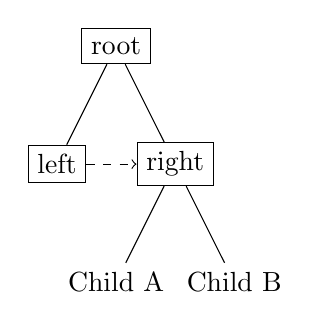
\begin{tikzpicture}[sibling distance=15mm]
    
  \node[rectangle,draw] {root}
    child {node[rectangle,draw] (left node) {left}}
    child {
        node[rectangle,draw] (right node) {right}
            child {node {Child A}}
		child {node {Child B}}
    };
  \draw[dashed,->] (left node) -- (right node);

\end{tikzpicture}
\end{center}

% %-----------------------------------------------------------

% %-----------------------------------------------------------
% % Timeline using TikZ
% % Designs obtained from https://stackoverflow.com/questions/217834/how-to-create-a-timeline-with-latex

% %Basic timeline

% \chronoperiodecoloralternation{orange, green,
% red, yellow, pink}
% \startchronology
% \chronoperiode[startdate=false]{0}{500}{}
% \chronoperiode[startdate=false]{500}{1000}{}
% \chronoperiode[startdate=false]{1000}{1500}{}
% \chronoperiode{1500}{1800}{Anything you want}
% \chronoperiode{1800}{1950}{18\textsuperscript{th} century}
% \chronoperiode{1950}{2100}{Anything you want}
% \stopchronology

% \setupchronology{startyear=1000,color=blue,stopdate=false}
% \setupchronoperiode{color=green}
% \setupchronoevent{textstyle=\it}
% \setupchronograduation[event]{markdepth=2cm}
% \startchronology
% \chronograduation{250}
% \chronoperiode{1050}{1450}{Anything you want}
% \chronoevent{1600}{Anything else}
% \chronoperiode{1800}{1899}{19\textsuperscript{th} century}
% \stopchronology

% \startchronology[startyear=-800,stopyear=500,
% color=green, height=3cm]
% \chronoperiode[color=orange,bottomdepth=1cm, topheight=2cm,
% textstyle=\it, dateselevation=-15pt, ifcolorbox=false,
% box=true]{-753}{-509}{Roman Royal period}
% \chronoperiode[color=cyan,startdate=false, textstyle=\bf,
% textdepth=35pt, bottomdepth=1cm, topheight=2cm,
% ifcolorbox=false, dateselevation=-15pt,
% box=true]{-509}{-27}{Roman Republic}
% \stopchronology

% %Straight Timeline
% \begin{tikzpicture}[remember picture, overlay, shift={(0,-3.5)}]

%   % Starting point at (0,0) on the page
%   \coordinate (start) at (0,0);

%   % Draw the first line: 25 degrees, 9cm length
%   \draw[color = blue!40, line join=round, line cap=round, shading angle=25, opacity=0.5, top color=blue!10, bottom color=blue!60] (start) -- ++(-30:9cm) coordinate (end1); 

%   % Draw the second line: -20 degrees, 9.5cm length
%   \draw[color = blue!40, line join=round, line cap=round, shading angle=-20, opacity=0.5, top color=blue!10, bottom color=blue!60] (start) -- ++(-26:9.5cm) coordinate (end2

%   % Fill the space between the lines with blue and reduced opacity
%   \begin{scope}
%     \path[clip] (start) -- (end1) -- (end2) -- cycle;
%     \shade[bottom color=blue!10, top color=blue!60, opacity=0.5] (start) rectangle (end2|-end1);
%   \end{scope}

%   % Draw ovals at the starting point
%   \draw[color = red, fill = red, opacity = 0.8, line width=0.01cm] (start) ++(-28:0.3cm) ellipse [x radius=0.05cm, y radius=0.012cm];
%   \draw[color = orange, fill = orange, opacity = 0.8, line width=0.01cm] (start) ++(-28:2.2cm) ellipse [x radius);=0.115cm, y radius=0.055cm];
%   \draw[color = yellow, fill = yellow, opacity = 0.8, line width=0.01cm] (start) ++(-28:3.8cm) ellipse [x radius=0.18cm, y radius=0.11cm];
%   \draw[color = green, fill = green, opacity = 0.8, line width=0.01cm] (start) ++(-27.95:6.2cm) ellipse [x radius=0.355cm, y radius=0.15cm];
%   \draw[color = teal, fill = teal, opacity = 0.8, line width=0.01cm] (start) ++(-27.95:8cm) ellipse [x radius=0.42cm, y radius=0.21cm];

%   % Draw ovals around the existing ovals
%   \draw[color = red, line width = 0.005cm] (start) ++(-28:0.3cm) ellipse [x radius=0.05*1.5cm, y radius=0.012cm*1.5];
%   \draw[color = orange, line width = 0.005cm] (start) ++(-28:2.2cm) ellipse [x radius=0.115cm*1.5, y radius=0.055cm*1.5];
%   \draw[color = yellow, line width = 0.005cm] (start) ++(-28:3.8cm) ellipse [x radius=0.18cm*1.5, y radius=0.11cm*1.5];
%   \draw[color = green, line width = 0.005cm] (start) ++(-27.95:6.2cm) ellipse [x radius=0.355cm*1.5, y radius=0.15cm*1.5];
%   \draw[color = teal, line width = 0.005cm] (start) ++(-27.95:8cm) ellipse [x radius=0.42cm*1.3, y radius=0.21cm*1.3];

%   % Draw perpendicular lines going up 3cm
%   \draw[color = red, dashed, opacity=0.8] (start) ++(-28:0.3cm) -- ++(90:3.5cm) node[right, scale = 0.9, color = red] {1997};
%   \draw[color = orange, dashed, opacity=0.8] (start) ++(-28:2.2cm) -- ++(90:3.5cm) node[right, scale=0.9, color = orange] {2004};
%   \draw[color = yellow, dashed, opacity=0.8] (start) ++(-28:3.8cm) -- ++(90:3.5cm) node[right, scale=0.9, color = yellow] {2005};
%   \draw[color = green, dashed, opacity=0.8] (start) ++(-27.95:6.2cm) -- ++(90:3.5cm) node[right, scale=0.9, color = green] {2007};
%   \draw[color = teal, dashed, opacity=0.8] (start) ++(-27.95:8cm) -- ++(90:3.5cm) node[right, scale=0.9, color = teal] {2010};

%   % Add text under the years
%   \node[right, color = black, scale = 0.5] (1) at ($(start) + (-28:0.4cm) + (90:3cm)$) {Lorem};
%   \node[right, color = black, scale = 0.5] (2) at ($(start) + (-28:0.4cm) + (90:2.8cm)$) {ipsum dolor};
%   \node[right, color = black, scale = 0.5] (3) at ($(start) + (-28:2.3cm) + (90:3cm)$) {Lorem};
%   \node[right, color = black, scale = 0.5] (4) at ($(start) + (-28:2.3cm) + (90:2.8cm)$) {ipsum dolor};
%   \node[right, color = black, scale = 0.5] (5) at ($(start) + (-28:3.9cm) + (90:3cm)$) {Lorem ipsum};
%   \node[right, color = black, scale = 0.5] (6) at ($(start) + (-28:3.9cm) + (90:2.8cm)$) {dolor sit};
%   \node[right, color = black, scale = 0.5] (7) at ($(start) + (-28:3.9cm) + (90:2.6cm)$) {amet};
%   \node[right, color = black, scale = 0.5] (8) at ($(start) + (-28:6.3cm) + (90:3cm)$) {Lorem};
%   \node[right, color = black, scale = 0.5] (9) at ($(start) + (-28:6.3cm) + (90:2.8cm)$) {ipsum};
%   \node[right, color = black, scale = 0.5] (10) at ($(start) + (-28:8.1cm) + (90:3cm)$) {Lorem};
%   \node[right, color = black, scale = 0.5] (11) at ($(start) + (-28:8.1cm) + (90:2.8cm)$) {ipsum dolor};
%   \node[right, color = black, scale = 0.5] (12) at ($(start) + (-28:8.1cm) + (90:2.6cm)$) {sit amet};

%   % Draw a box around the text nodes with the same opacity
%   \node[draw, line width = 0.005cm, rounded corners, scale = 0.8, fit={(1) (2)}] {};
%   \node[draw, line width = 0.005cm, rounded corners, scale = 0.8, fit={(3) (4)}] {};
%   \node[draw, line width = 0.005cm, rounded corners, scale = 0.8, fit={(5) (6) (7)}] {};
%   \node[draw, line width = 0.005cm, rounded corners, scale = 0.8, fit={(8) (9)}] {};
%   \node[draw, line width = 0.005cm, rounded corners, scale = 0.8, fit={(10) (11) (12)}] {};
  
% \end{tikzpicture}

% \newpage

% %Curved Timeline
% \begin{tikzpicture}[remember picture, overlay, shift={(8,-3)}]

%   %Define control points for the first S-shaped curve
%   \coordinate (start) at (-4, 0);
%   \coordinate (control1) at (6, -3);
%   \coordinate (middle) at (0, -7);
%   \coordinate (end1) at (-6, -11);

%   % Draw the first S-shaped curve
%   \draw(start) .. controls (control1) .. (middle) .. controls (middle) and (end1) .. (end1);

%   % Optional: Add labels to the control points for the first curve
%   %\filldraw [purple] (start) circle (2pt) node[below] {Start};
%   %\filldraw [red] (control1) circle (2pt) node[left] {Control 1};
%   %\filldraw [red] (middle) circle (2pt) node[above] {Middle};
%   %\filldraw [red] (end1) circle (2pt) node[below] {End 1};

%   % Define control points for the second S-shaped curve
%   \coordinate (control3) at (8, -2.5);
%   \coordinate (middle2) at (4, -6.5);
%   \coordinate (end2) at (-3, -14);

%   % Draw the second S-shaped curve with an arrow at the end
%   \draw (start) .. controls (control3) .. (middle2) .. controls (middle2) and (end2) .. (end2);

%   % Optional: Add labels to the control points for the second curve
%   %\filldraw [blue] (control3) circle (2pt) node[right] {Control 3};
%   %\filldraw [blue] (middle2) circle (2pt) node[below] {Middle 2};
%   %\filldraw [blue] (end2) circle (2pt) node[above] {End 2};

%   %General coordinates
%   \coordinate (arrow1) at ($(end1) + (-1, +1)$);
%   \coordinate (arrow2) at ($(end2) + (+1, -1)$);
%   \coordinate (arrow3) at ($(arrow2) + (-5.3, 0)$);

%   % Optional: Add labels to the control points for the arrow head
%   %\filldraw [green] (arrow1) circle (2pt) node[below] {Arrow 1};
%   %\filldraw [green] (arrow2) circle (2pt) node[above] {Arrow 2};
%   %\filldraw [green] (arrow3) circle (2pt) node[above] {Arrow 3};

%   %Draw the arrow head
%   \draw (end1) -- (arrow1) -- (arrow3) -- (arrow2) -- (end2);

%  %Shade the region between the two curves
%  \begin{scope}
%     \shade[bottom color=blue!10, top color=blue!60, opacity=0.8] 
%       (arrow3) -- (arrow2) -- (end2) -- (middle2) .. controls (control3) .. (start) .. controls (control1) .. (middle) .. controls (middle) and (end1) .. (end1) -- (arrow1) -- (arrow3) -- cycle;
%   \end{scope}

%   % Define control points for the curved path
%   \coordinate (pathControl) at ($(control1)!0.5!(control3)$);
%   \coordinate (pathMiddle) at ($(middle)!0.5!(middle2)$);
%   \coordinate (pathEnd) at (arrow3);
%   \coordinate (pathEnd2) at ($(end1)!0.5!(end2)$);

%   % Draw the curved path
%   %\filldraw [yellow] (pathControl) circle (2pt) node[below] {Path Control};
%   %\filldraw [yellow] (pathMiddle) circle (2pt) node[below] {Path Middle};
%   %\filldraw [yellow] (pathEnd) circle (2pt) node[below] {Path End};
%   %\filldraw [yellow] (pathEnd2) circle (2pt) node[below] {Path End2};
%   %\draw[red] (start) .. controls (pathControl) .. (pathMiddle) .. controls (pathMiddle) and (pathEnd) .. (pathEnd2);
%   %\draw[blue] (pathEnd2) -- (pathEnd);

%   % Draw ovals at the starting point
%   \draw[color = red, fill = red, opacity = 0.8, line width=0.01cm] ($(start) + (0.806, -0.2)$) ellipse [x radius=0.098cm, y radius=0.0225cm];
%   \draw[color = orange, fill = orange, opacity = 0.8, line width=0.01cm] ($(start) + (4.2, -1.074)$) ellipse [x radius=0.436cm, y radius=0.155cm];
%   \draw[color = yellow, fill = yellow, opacity = 0.8, line width=0.01cm] ($(start) + (6.85, -1.84)$) ellipse [x radius=0.77cm, y radius=0.27cm];
%   \draw[color = green, fill = green, opacity = 0.8, line width=0.01cm] ($(start) + (9.23, -3.55)$) ellipse [x radius=1.135cm, y radius=0.5cm];
%   \draw[color = teal, fill = teal, opacity = 0.8, line width=0.01cm] ($(start) + (7.31, -5.8)$) ellipse [x radius=1.22cm, y radius=0.65cm];
%   \draw[color = blue, fill = blue, opacity = 0.8, line width=0.01cm] ($(start) + (5.02, -7.7)$) ellipse [x radius=1.72cm, y radius=0.75cm];
%   \draw[color = purple, fill = purple, opacity = 0.8, line width=0.01cm] ($(start) + (2.1, -10.111)$) ellipse [x radius=2.36cm, y radius=0.95cm];

%   % Draw ovals around the existing ovals with the same ratios
%   \draw[color=red, line width=0.005cm] ($(start) + (0.806, -0.2)$) ellipse [x radius=0.098cm*1.575, y radius=0.0225cm*1.575];
%   \draw[color=orange, line width=0.005cm] ($(start) + (4.2, -1.074)$) ellipse [x radius=0.436cm*1.5, y radius=0.155cm*1.5];
%   \draw[color = yellow, line width = 0.005cm] ($(start) + (6.85, -1.84)$) ellipse [x radius=0.77cm*1.3, y radius=0.27cm*1.3];
%   \draw[color = green, line width = 0.005cm] ($(start) +(9.23, -3.55)$) ellipse [x radius=1.135cm*1.3, y radius=0.5cm*1.3];
%   \draw[color = teal, line width = 0.005cm] ($(start) + (7.31, -5.8)$) ellipse [x radius=1.22cm*1.3, y radius=0.65cm*1.3];
%   \draw[color = blue, line width = 0.005cm] ($(start) + (5.02, -7.7)$) ellipse [x radius=1.72cm*1.25, y radius=0.75cm*1.25];
%   \draw[color = purple, line width = 0.005cm] ($(start) + (2.1, -10.111)$) ellipse [x radius=2.36cm*1.2, y radius=0.95cm*1.2];

%   % Draw perpendicular lines going up 3cm
%   \draw[color = red, dashed, opacity = 1] ($(start) + (0.806, -0.2)$) -- ++(90:3.5cm) node[right, scale = 0.9, color = red] {1997};
%   \draw[color = orange, dashed, opacity = 1] ($(start) + (4.2, -1.074)$) -- ++(90:3.5cm) node[right, scale = 0.9, color = orange] {2004};
%   \draw[color = yellow, dashed, opacity = 1] ($(start) + (6.85, -1.84)$) -- ++(90:3.5cm) node[right, scale = 0.9, color = yellow] {2005};
%   \draw[color = green, dashed, opacity = 1] ($(start) + (9.23, -3.55)$) -- ++(-90:3.5cm)  node[right, scale = 0.9, color = green] {2007};
%   \draw[color = teal, dashed, opacity = 1] ($(start) + (7.31, -5.8)$) -- ++(-90:3.5cm) node[right, scale = 0.9, color = teal] {2010};
%   \draw[color = blue, dashed, opacity = 1] ($(start) + (5.02, -7.7)$) -- ++(-90:4.5cm) node[right, scale = 0.9, color = blue] {2013};
%   \draw[color = purple, dashed, opacity = 1] ($(start) + (2.1, -10.111)$) -- ++(-90:4.5cm) node[right, scale = 0.9, color = purple] {2017};

%   % Add text under the years
%   \node[right, color = black, scale = 1] (1) at ($(start) + (0.87, -0.2)  + (90:2.8cm)$) {Lorem};
%   \node[right, color = black, scale = 1] (2) at ($(start) + (0.87, -0.32)  + (90:2.4cm)$) {ipsum dolor};
%   \node[right, color = black, scale = 1] (3) at ($(start) + (4.27, -1.074)  + (90:2.8cm)$) {Lorem};
%   \node[right, color = black, scale = 1] (4) at ($(start) + (4.27, -1.074) + (90:2.4cm)$) {ipsum dolor};
%   \node[right, color = black, scale = 1] (5) at ($(start) + (6.95, -1.84) + (90:2.8cm)$) {Lorem};
%   \node[right, color = black, scale = 1] (6) at ($(start) + (6.95, -1.84)+ (90:2.4cm)$) {dolor sit};
%   \node[right, color = black, scale = 1] (7) at ($(start) + (6.95, -1.84) + (90:2cm)$) {amet};
%   \node[right, color = black, scale = 1] (8) at ($(start) + (9.38, -3.55) + (-90:2.4cm)$) {Lorem};
%   \node[right, color = black, scale = 1] (9) at ($(start) + (9.38, -3.55) + (-90:2.8cm)$) {ipsum};
%   \node[right, color = black, scale = 1] (10) at ($(start) + (7.36, -5.8) + (-90:2cm)$) {Lorem ipsum};
%   \node[right, color = black, scale = 1] (11) at ($(start) + (7.36, -5.8) + (-90:2.4cm)$) {dolor sit};
%   \node[right, color = black, scale = 1] (12) at ($(start) + (7.36, -5.8) + (-90:2.8cm)$) {amet};
%   \node[right, color = black, scale = 1] (13) at ($(start) + (5.09, -7.7) + (-90:3cm)$) {Lorem ipsum};
%   \node[right, color = black, scale = 1] (14) at ($(start) + (5.09, -7.7) + (-90:3.4cm)$) {dolor sit};
%   \node[right, color = black, scale = 1] (15) at ($(start) + (5.09, -7.7) + (-90:3.8cm)$) {amet};
%   \node[right, color = black, scale = 1] (16) at ($(start) + (2.25, -10.111) + (-90:3.4cm)$) {Lorem};
%   \node[right, color = black, scale = 1] (17) at ($(start) + (2.25, -10.111) + (-90:3.8cm)$) {ipsum};

%   % Draw a box around the text nodes with the same opacity
%   \node[draw, line width = 0.005cm, rounded corners, scale = 0.85, fit={(1) (2)}] {};
%   \node[draw, line width = 0.005cm, rounded corners, scale = 0.85, fit={(3) (4)}] {};
%   \node[draw, line width = 0.005cm, rounded corners, scale = 0.85, fit={(5) (6) (7)}] {};
%   \node[draw, line width = 0.005cm, rounded corners, scale = 0.85, fit={(8) (9)}] {};
%   \node[draw, line width = 0.005cm, rounded corners, scale = 0.85, fit={(10) (11) (12)}] {};
%   \node[draw, line width = 0.005cm, rounded corners, scale = 0.85, fit={(13) (14) (15)}] {};
%   \node[draw, line width = 0.005cm, rounded corners, scale = 0.85, fit={(16) (17)}] {};

% \end{tikzpicture}

% %-----------------------------------------------------------

\newpage

%References
\bibliographystyle{cmj}
\bibliography{cmjbib}

\end{document}
